\documentclass[../master/master.tex]{subfiles}

\begin{document}

\renewcommand{\lecturenum}{F}
\renewcommand{\lecturedate}{Spring 2026}
\renewcommand{\lecturetopic}{Filler: Missing Concepts from Lectures 1--6}

\section{Filler: Missing Concepts}

\begin{lecturesummary}
\textbf{Overview:} Four concepts that appear in the midterm review but are absent from the lecture notes. These fill gaps in Lectures 4 and 5.
\end{lecturesummary}

%======================================================================
\subsection{Interior of a Set (Lecture 4 gap)}
%======================================================================

\begin{summarybox}
\textbf{Section Overview:} The interior is the dual of closure. Closure grows a set outward to include its boundary; interior shrinks a set inward to its open core. Lecture 4 defines closure ($\overline{E}$) and limit points ($E'$) but omits the interior ($E^\circ$).
\end{summarybox}

\begin{definition}
The \defn{interior} of a set $E \subseteq X$ is the largest open set contained in $E$:
\[
    E^\circ = \bigcup \{ U \subseteq X : U \text{ is open and } U \subseteq E \}.
\]
\end{definition}

\textbf{Equivalent characterization (metric spaces):} $x \in E^\circ$ if and only if there exists $\delta > 0$ such that $B(x, \delta) \subseteq E$.

Intuitively, $x$ is in the interior of $E$ if $x$ has ``room around it'' that stays entirely inside $E$.

\begin{example}
Let $E = [0, 1] \subset \R$.
\begin{itemize}
    \item $E^\circ = (0, 1)$: any point in $(0,1)$ has a ball fitting inside $[0,1]$, but $0$ and $1$ do not (every ball around them escapes $[0,1]$).
    \item $\overline{E} = [0, 1]$: already closed.
\end{itemize}

Let $E = (0, 1) \subset \R$.
\begin{itemize}
    \item $E^\circ = (0, 1)$: already open.
    \item $\overline{E} = [0, 1]$: adds the limit points $0$ and $1$.
\end{itemize}

Let $E = \Q \subset \R$.
\begin{itemize}
    \item $E^\circ = \emptyset$: no ball $(x - \delta, x + \delta)$ consists entirely of rationals (irrationals are everywhere).
    \item $\overline{E} = \R$: every real number is a limit point of $\Q$.
\end{itemize}
\end{example}

\subsubsection*{Duality with Closure}

Interior and closure are related by complementation:
\[
    (X \setminus E)^\circ = X \setminus \overline{E}, \qquad \overline{X \setminus E} = X \setminus E^\circ.
\]

\begin{center}
\renewcommand{\arraystretch}{1.3}
\begin{tabular}{|c|c|c|}
\hline
\textbf{Property} & \textbf{Interior $E^\circ$} & \textbf{Closure $\overline{E}$} \\
\hline
Definition & Largest open set $\subseteq E$ & Smallest closed set $\supseteq E$ \\
Characterization & $\exists\; B(x,\delta) \subseteq E$ & every nbhd of $x$ meets $E$ \\
Always satisfies & $E^\circ \subseteq E$ & $E \subseteq \overline{E}$ \\
$E$ is open $\iff$ & $E^\circ = E$ & --- \\
$E$ is closed $\iff$ & --- & $\overline{E} = E$ \\
\hline
\end{tabular}
\end{center}

\begin{notebox}
\textbf{The boundary.} With both interior and closure in hand, we can define the \defn{boundary} of $E$:
\[
    \partial E = \overline{E} \setminus E^\circ.
\]
These are the points that are ``on the edge'' --- in the closure but not in the interior. For example, $\partial [0,1] = \{0, 1\}$ and $\partial \Q = \R$.
\end{notebox}

\newpage
%======================================================================
\subsection{Dense Sets (Lecture 4 gap)}
%======================================================================

\begin{summarybox}
\textbf{Section Overview:} Lecture 2 proves that $\Q$ is dense in $\R$ (between any two reals there is a rational), but the general topological definition of ``dense'' never appears in the notes.
\end{summarybox}

\begin{definition}
A subset $E$ of a topological space $X$ is \defn{dense} in $X$ if $\overline{E} = X$.
\end{definition}

\textbf{Equivalent characterizations:}
\begin{enumerate}
    \item Every nonempty open set in $X$ contains a point of $E$.
    \item Every point of $X$ is either in $E$ or is a limit point of $E$ (i.e., $X = E \cup E'$).
    \item In a metric space: for every $x \in X$ and every $\eps > 0$, $B(x, \eps) \cap E \neq \emptyset$.
\end{enumerate}

\begin{example}
$\Q$ is dense in $\R$: $\overline{\Q} = \R$. This is precisely the density theorem from Lecture 2 restated in topological language --- for any $a < b$, the open interval $(a, b)$ contains a rational.
\end{example}

\begin{example}
The irrationals $\R \setminus \Q$ are also dense in $\R$. Between any two reals, there is an irrational (e.g., take a rational $q$ between them and add $\frac{\sqrt{2}}{n}$ for large $n$). So $\overline{\R \setminus \Q} = \R$ as well.
\end{example}

\begin{example}
$\Z$ is \emph{not} dense in $\R$: the open interval $(0.1, 0.9)$ contains no integers. Equivalently, $\overline{\Z} = \Z \neq \R$ (each integer is isolated).
\end{example}

\begin{remark}
The phrase ``$\R$ is the completion of $\Q$'' (from the midterm review) combines two ideas: $\Q$ is dense in $\R$ (the rationals are spread everywhere), and $\R$ has the LUBP (all the gaps are filled). $\R$ is the smallest ordered field containing $\Q$ with no gaps.
\end{remark}

\newpage
%======================================================================
\subsection{Convergent Sequences are Bounded (Lecture 4 gap)}
%======================================================================

\begin{summarybox}
\textbf{Section Overview:} Lecture 4 defines both convergence and boundedness, but never states their relationship. This is a basic and frequently used fact.
\end{summarybox}

\begin{theorem}
If $(x_n) \to y$ in a metric space $(X, d)$, then the sequence $(x_n)$ is bounded: there exists $M > 0$ such that $d(x_n, y) \leq M$ for all $n$.
\end{theorem}

\begin{proof}
Apply the definition of convergence with $\eps = 1$: there exists $N \in \N$ such that $d(x_n, y) < 1$ for all $n \geq N$.

\textbf{The tail is bounded:} For $n \geq N$, $d(x_n, y) < 1$.

\textbf{The head is finite:} The terms $x_1, \ldots, x_{N-1}$ are finitely many, so
\[
    M_0 = \max\{d(x_1, y), \, d(x_2, y), \, \ldots, \, d(x_{N-1}, y)\}
\]
is finite.

\textbf{Combine:} Let $M = \max(M_0, 1)$. Then $d(x_n, y) \leq M$ for all $n \in \N$.
\end{proof}

\begin{center}
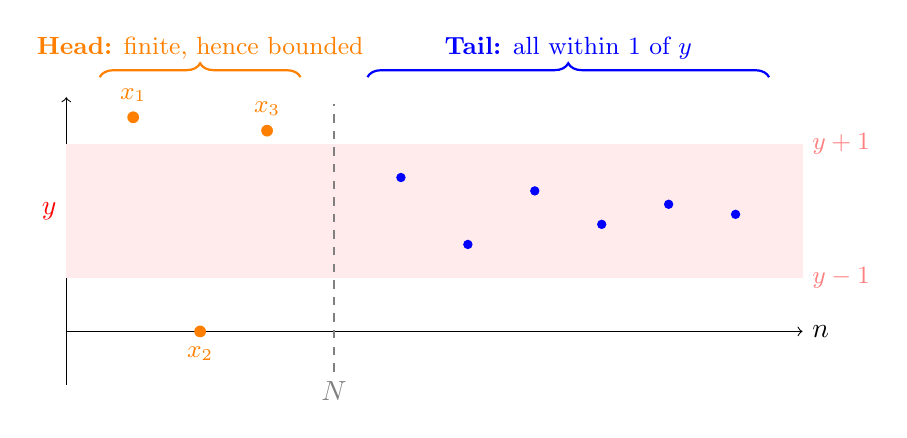
\begin{tikzpicture}[scale=0.85]
    \draw[->] (0,0) -- (11,0) node[right] {$n$};
    \draw[->] (0,-0.8) -- (0,3.5);

    % The limit
    \draw[dashed, red, thick] (0,1.8) -- (11,1.8);
    \node[red, left] at (0,1.8) {$y$};

    % Epsilon band (eps = 1)
    \fill[red!8] (0,0.8) rectangle (11,2.8);
    \node[red!50, right] at (11, 2.8) {\small $y + 1$};
    \node[red!50, right] at (11, 0.8) {\small $y - 1$};

    % Head: finitely many terms
    \fill[orange] (1, 3.2) circle (2.5pt) node[above=2pt] {\small $x_1$};
    \fill[orange] (2, 0.0) circle (2.5pt) node[below=2pt] {\small $x_2$};
    \fill[orange] (3, 3.0) circle (2.5pt) node[above=2pt] {\small $x_3$};

    % N marker
    \draw[thick, gray, dashed] (4,-0.6) -- (4,3.4);
    \node[gray, below] at (4,-0.6) {$N$};

    % Tail: all within 1 of y
    \fill[blue] (5, 2.3) circle (2pt);
    \fill[blue] (6, 1.3) circle (2pt);
    \fill[blue] (7, 2.1) circle (2pt);
    \fill[blue] (8, 1.6) circle (2pt);
    \fill[blue] (9, 1.9) circle (2pt);
    \fill[blue] (10, 1.75) circle (2pt);

    % Braces
    \draw[thick, orange, decorate, decoration={brace, amplitude=5pt}] (0.5,3.8) -- (3.5,3.8);
    \node[orange, above=3pt] at (2, 3.8) {\small \textbf{Head:} finite, hence bounded};

    \draw[thick, blue, decorate, decoration={brace, amplitude=5pt}] (4.5,3.8) -- (10.5,3.8);
    \node[blue, above=3pt] at (7.5, 3.8) {\small \textbf{Tail:} all within $1$ of $y$};
\end{tikzpicture}
\end{center}

\begin{notebox}
\textbf{Pattern: head--tail decomposition.} This is a common technique in analysis. Convergence gives you control over the \emph{tail} (all terms past some $N$). The \emph{head} (finitely many initial terms) is automatically tamed because any finite set is bounded. Taking the max combines both. The same idea appears when proving that convergent sequences in $\R$ are Cauchy, and in many other arguments.
\end{notebox}

\newpage
%======================================================================
\subsection{Sequential Compactness (Lecture 5 gap)}
%======================================================================

\begin{summarybox}
\textbf{Section Overview:} Lecture 5 proves Heine--Borel condition (3) --- ``every infinite subset has a limit point'' --- but never names or formally defines \defn{sequential compactness}. This is the subsequence-based characterization of compactness.
\end{summarybox}

\begin{definition}
A set $K$ in a metric space is \defn{sequentially compact} if every sequence in $K$ has a subsequence that converges to a point in $K$.
\end{definition}

\subsubsection*{Relation to Heine--Borel}

In $\R^n$, the Heine--Borel theorem (Lecture 5) gives three equivalent characterizations of compactness. Sequential compactness is essentially condition (3):

\begin{center}
\renewcommand{\arraystretch}{1.5}
\begin{tabular}{|c|p{9cm}|}
\hline
\textbf{(1)} & $K$ is \textbf{closed and bounded} \\
\hline
\textbf{(2)} & $K$ is \textbf{compact}: every open cover has a finite subcover \\
\hline
\textbf{(3)} & Every \textbf{infinite subset} of $K$ has a limit point in $K$ $\;\Longleftrightarrow\;$ $K$ is sequentially compact \\
\hline
\end{tabular}
\end{center}

\subsubsection*{Why (3) implies sequential compactness}

Given a sequence $(x_n)$ in $K$:
\begin{itemize}
    \item If infinitely many terms are distinct, the set $\{x_n\}$ is an infinite subset of $K$, so it has a limit point $p \in K$ by condition (3). Since every neighborhood of $p$ contains infinitely many points of $\{x_n\}$ (Lecture 4), we can extract a subsequence converging to $p$.
    \item If only finitely many values appear, some value repeats infinitely often, giving a constant (hence convergent) subsequence.
\end{itemize}

\begin{center}
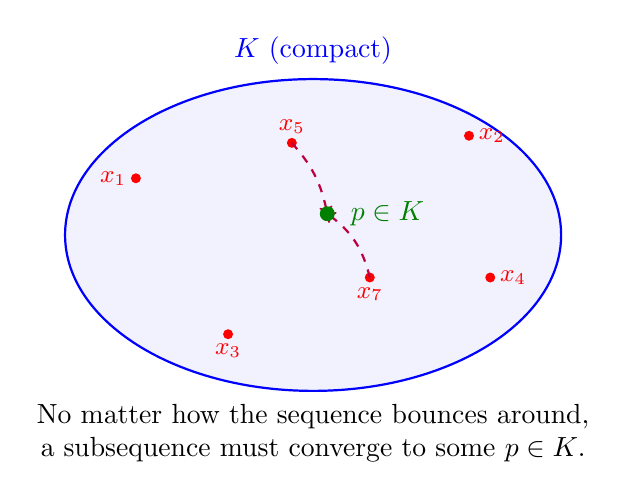
\begin{tikzpicture}[scale=0.9]
    % Compact set
    \draw[thick, blue, fill=blue!5] (0,0) ellipse (3.5 and 2.2);
    \node[blue] at (0, 2.6) {$K$ (compact)};

    % Sequence terms bouncing around
    \fill[red] (-2.5, 0.8) circle (2pt) node[left] {\small $x_1$};
    \fill[red] (2.2, 1.4) circle (2pt) node[right] {\small $x_2$};
    \fill[red] (-1.2, -1.4) circle (2pt) node[below] {\small $x_3$};
    \fill[red] (2.5, -0.6) circle (2pt) node[right] {\small $x_4$};
    \fill[red] (-0.3, 1.3) circle (2pt) node[above] {\small $x_5$};
    \fill[red] (0.8, -0.6) circle (2pt) node[below] {\small $x_7$};

    % Subsequence converging
    \draw[->, thick, purple, dashed] (-0.3, 1.3) to[bend left=15] (0.2, 0.3);
    \draw[->, thick, purple, dashed] (0.8, -0.6) to[bend right=20] (0.2, 0.3);

    % Limit point
    \fill[green!50!black] (0.2, 0.3) circle (3pt);
    \node[green!50!black, right=5pt] at (0.2, 0.3) {$p \in K$};

    \node[align=center] at (0, -2.8) {No matter how the sequence bounces around,\\
    a subsequence must converge to some $p \in K$.};
\end{tikzpicture}
\end{center}

\subsubsection*{Intuition: Why must a subsequence converge?}

The sequence itself does \emph{not} converge --- it can bounce around wildly. The claim is that you can always \textbf{cherry-pick} a well-behaved subsequence from the chaos.

\begin{example}
Consider a sequence bouncing randomly in $[0,1]$:
\[
    x_1 = 0.7, \quad x_2 = 0.2, \quad x_3 = 0.95, \quad x_4 = 0.11, \quad x_5 = 0.73, \quad x_6 = 0.71, \quad x_7 = 0.698, \quad \ldots
\]
This sequence does not converge. But the subsequence $x_1, x_5, x_6, x_7 = 0.7, 0.73, 0.71, 0.698, \ldots$ is clustering near $0.7$. Sequential compactness guarantees that such a clustering subsequence \emph{always} exists.
\end{example}

\textbf{The bisection argument (why it must work).} We use the same bisection technique from the proof that $[a,b]$ is compact (Lecture 5):

\begin{enumerate}
    \item Split $[0,1]$ into two halves: $[0, \tfrac{1}{2}]$ and $[\tfrac{1}{2}, 1]$. Infinitely many terms of the sequence must land in at least one half --- you cannot split infinitely many terms into two finite piles. Pick that half; call it $I_1$.

    \item Split $I_1$ in half again. Again, infinitely many terms land in at least one quarter. Pick it; call it $I_2$.

    \item Repeat. At each step, we get a nested interval $I_n$ of length $1/2^n$ containing infinitely many terms of the sequence.
\end{enumerate}

This gives nested closed intervals:
\[
    [0,1] \supset I_1 \supset I_2 \supset I_3 \supset \cdots, \qquad |I_n| = \frac{1}{2^n}.
\]
Since each $I_n$ contains infinitely many terms, we can pick one term $x_{n_k}$ from each $I_k$ (with strictly increasing indices). The nested intervals theorem gives a point $p \in \bigcap_n I_n$, and since the intervals shrink to length $0$, we have $x_{n_k} \to p$.

\begin{center}
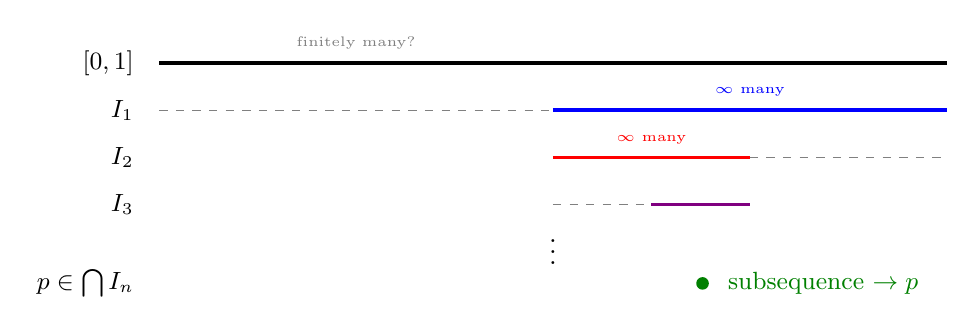
\begin{tikzpicture}[scale=10]
    % I_0 = [0, 1]
    \draw[very thick] (0,0) -- (1,0);
    \node[left] at (-0.02,0) {\small $[0,1]$};

    % I_1 = [0.5, 1] (say right half has more)
    \draw[very thick, blue] (0.5,-0.06) -- (1,-0.06);
    \draw[gray, dashed] (0,-0.06) -- (0.5,-0.06);
    \node[left] at (-0.02,-0.06) {\small $I_1$};
    \node[gray, above] at (0.25, 0.005) {\tiny finitely many?};
    \node[blue, above] at (0.75, -0.055) {\tiny $\infty$ many};

    % I_2 = [0.5, 0.75]
    \draw[very thick, red] (0.5,-0.12) -- (0.75,-0.12);
    \draw[gray, dashed] (0.75,-0.12) -- (1,-0.12);
    \node[left] at (-0.02,-0.12) {\small $I_2$};
    \node[red, above] at (0.625, -0.115) {\tiny $\infty$ many};

    % I_3 = [0.625, 0.75]
    \draw[very thick, violet] (0.625,-0.18) -- (0.75,-0.18);
    \draw[gray, dashed] (0.5,-0.18) -- (0.625,-0.18);
    \node[left] at (-0.02,-0.18) {\small $I_3$};

    % Dots
    \node at (0.5,-0.23) {$\vdots$};

    % Limit point
    \fill[green!50!black] (0.69,-0.28) circle (0.008);
    \node[left] at (-0.02,-0.28) {\small $p \in \bigcap I_n$};
    \node[green!50!black, right] at (0.71,-0.28) {\small subsequence $\to p$};
\end{tikzpicture}
\end{center}

\begin{notebox}
\textbf{Why compactness (closed + bounded) is essential.}
\begin{itemize}
    \item \textbf{Bounded} prevents terms from ``escaping to infinity.'' The sequence is trapped in a box, so it \emph{must} pile up somewhere. Without boundedness: $x_n = n$ in $\R$ has no convergent subsequence.
    \item \textbf{Closed} ensures the limit point stays inside $K$. Without closedness: $x_n = 1/n$ in $(0,1)$ has the subsequence converging to $0$, but $0 \notin (0,1)$.
\end{itemize}
Together, closed and bounded mean the terms are trapped \emph{and} the limit cannot escape. That is why compactness forces a convergent subsequence to exist.
\end{notebox}

\subsubsection*{Why This Matters}

Sequential compactness is the mechanism behind several major theorems:
\begin{itemize}
    \item \textbf{Extreme Value Theorem (Lecture 6):} To show $f$ attains its max on $K$, take a sequence with $f(x_n) \to \sup f(K)$. Sequential compactness gives a convergent subsequence $x_{n_k} \to p \in K$, and continuity gives $f(p) = \sup f(K)$.
    \item \textbf{Bolzano--Weierstrass (Lecture 5):} Every bounded sequence in $\R^n$ has a convergent subsequence. This follows immediately: a bounded sequence lives in a closed box $[-M, M]^n$, which is compact, hence sequentially compact.
    \item \textbf{Uniform continuity (Lecture 6):} The proof that continuous functions on compact sets are uniformly continuous uses the finite subcover definition, but the intuition is sequential: if uniform continuity fails, you can build two sequences contradicting compactness.
\end{itemize}

\end{document}
